\documentclass{sciposter}
\usepackage{lipsum}
\usepackage{epsfig}
\usepackage{subfig}
\usepackage{amsmath}
\usepackage{amssymb}
\usepackage{multicol}
\usepackage{graphicx,url}
\usepackage[english,american]{babel}   
\usepackage[utf8]{inputenc}
\newtheorem{Def}{Definition}

\title{\begin{Huge}
		Residual gravity anomaly of Barreirinhas basin through Gemma crustal modeling
	\end{Huge}}
\author{Nelson Ribeiro Filho, Cristiano Martins \& Boris Freimann}
\institute 
{Observatório Nacional (ON/MCTI) \& 
	Universidade Federal do Pará (UFPA)}
\email{Correspond to: {nelsondelimar}{@gmail.com}}
\rightlogo[1.]{figures/logo-on.png}
\leftlogo[1.]{figures/logo01.png}

\begin{document}
	
	\conference{
		\begin{Large}
			{\bf XV CGCH 2018:} XV Congreso Geológico Chileno - 18 Al 23 de Noviembre de 2018 - Universidade de Concepción, Concepción, Chile
		\end{Large}}
	
	\maketitle

	\begin{multicols}{3}

	\section*{\large Introduction}
	\PARstart{G}{ravity signal} is a composition of all nearby sources beneath Earth's surface, since shallow heterogeneities from deep crustal structures \cite{blakely1996potential}. However the crust-mantle boundary (\textbf{Moho}) can cause a significant amplitude changes. It turns harder gravity interpretation and its dependence on the separation of both existing signals.
		
	Many regional-residual techniques have been proposed: spectral analysis \cite{spector1970statistical}; wavelet analysis \cite{fedi1998wavelet}; and fitting a polynomial \cite{beltrao1991robust}. An additional possibility is incorporate the crustal modeling. One way to perform it is by assuming crust depth and density are known. 
		
	We compared robust polynomial fitting and spectral analysis with crustal modeling by using crust model of Moho relief, density and geological provinces from GEMMA \cite{sampietro2013gemma}.
		
	\section*{\large Gravity crustal modeling}
	We delimited a region on $x-y$ plane that contains the crust area and its volume was selected by crustal thickness. We discretized it with $M$ elementary prisms with dimension $(dx, dy, dz)$ displayed in both directions until thickness is fully filled. Density between crust and mantle is known and homogeneous.
	
	We calculated gravity component at each observation point $P$ due to all 3D rectangular prisms \cite{blakely1996potential}:
	\begin{small}
		$$
		\mathbf{g_z}_i = \gamma \rho \int_{z_1}^{z_2} \int_{y_1}^{y_2} \int_{x_1}^{x_2}
		\dfrac{(z - z^{'}) \, dx^{'}dy^{'}dz^{'}}
		{\left[(x - x^{'})^2 + 
		(y - y^{'})^2 + 
		(z - z^{'})^2\right]^{\frac{3}{2}}}
		$$
	\end{small}
	where $\gamma$ is the universal gravitational constant and $\rho$ is the density.
	
	The density, top and bottom of crust and sediment thickness are  provided by GEMMA model. The final signal contains the gravity anomaly of all heterogeneous crust, sediments layers and the water sheets correction. The final gravity signal is written by:
	\begin{small}
		$$
		\mathbf{G_z} = 
		\mathbf{g_z}_{crust} + 
		\mathbf{g_z}_{sed} + 
		\mathbf{g_z}_{water}
		$$
	\end{small}
	To calculate the residual anomaly, which is related to the sedimentary basin, we evaluated the difference between observed gravity signal and the regional computed.
	
	\section*{\large Study area and geological context}
	We selected Barreirinhas Basin as study area, which is included in \textbf{new petroleum frontier} group and is located at Brazilian equatorial margin (figure \ref{fig0}). This region was formed by extension and strike-slip movements related to South Atlantic Ocean opening that resulted in several coastal basins \cite{almeida2009quaternary,soaresjunior2008evolucao}.
	
	\begin{figure}
		\begin{center}
			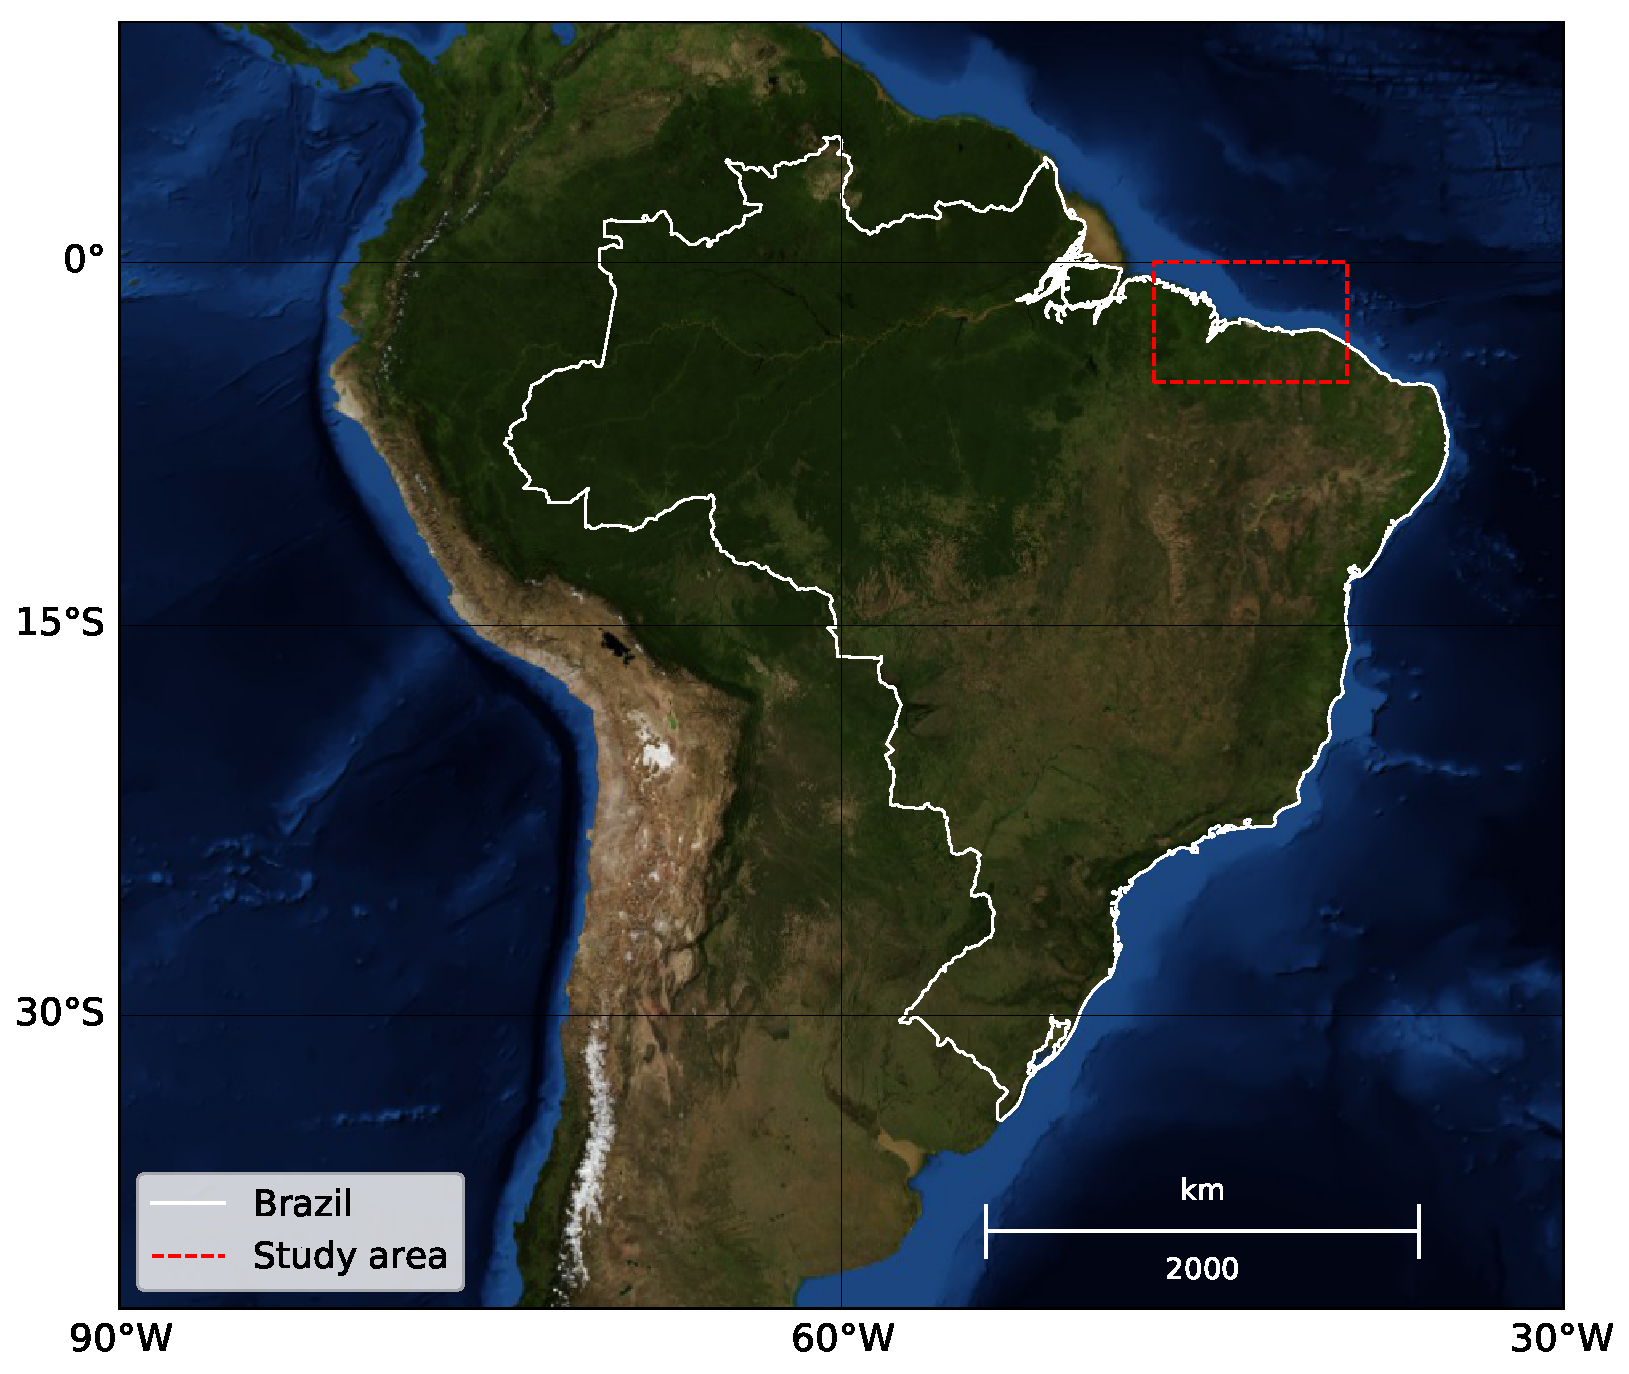
\includegraphics[width=0.9\textwidth]{figures/figure01a-location.pdf}
		\end{center}
		\caption{Brazilian continental margin. Red box represents our study area: Barreirinhas basin continental part.}
		\label{fig0}
	\end{figure}
	
	Barreirinhas basin forms a deep grabens system limited by normal faults with NW-SE orientation. These characteristics suggest this area was strongly affected by tectonics along normal faults \cite{almeida2009quaternary}. Its main depocenter stayed over Sobradinho Fault and shows sedimentary pile that reaches $1.6$ km of thickness (see figure \ref{fig1}).
	
	\begin{figure}[ht!]
	\begin{center}
	\subfigure[]{%
	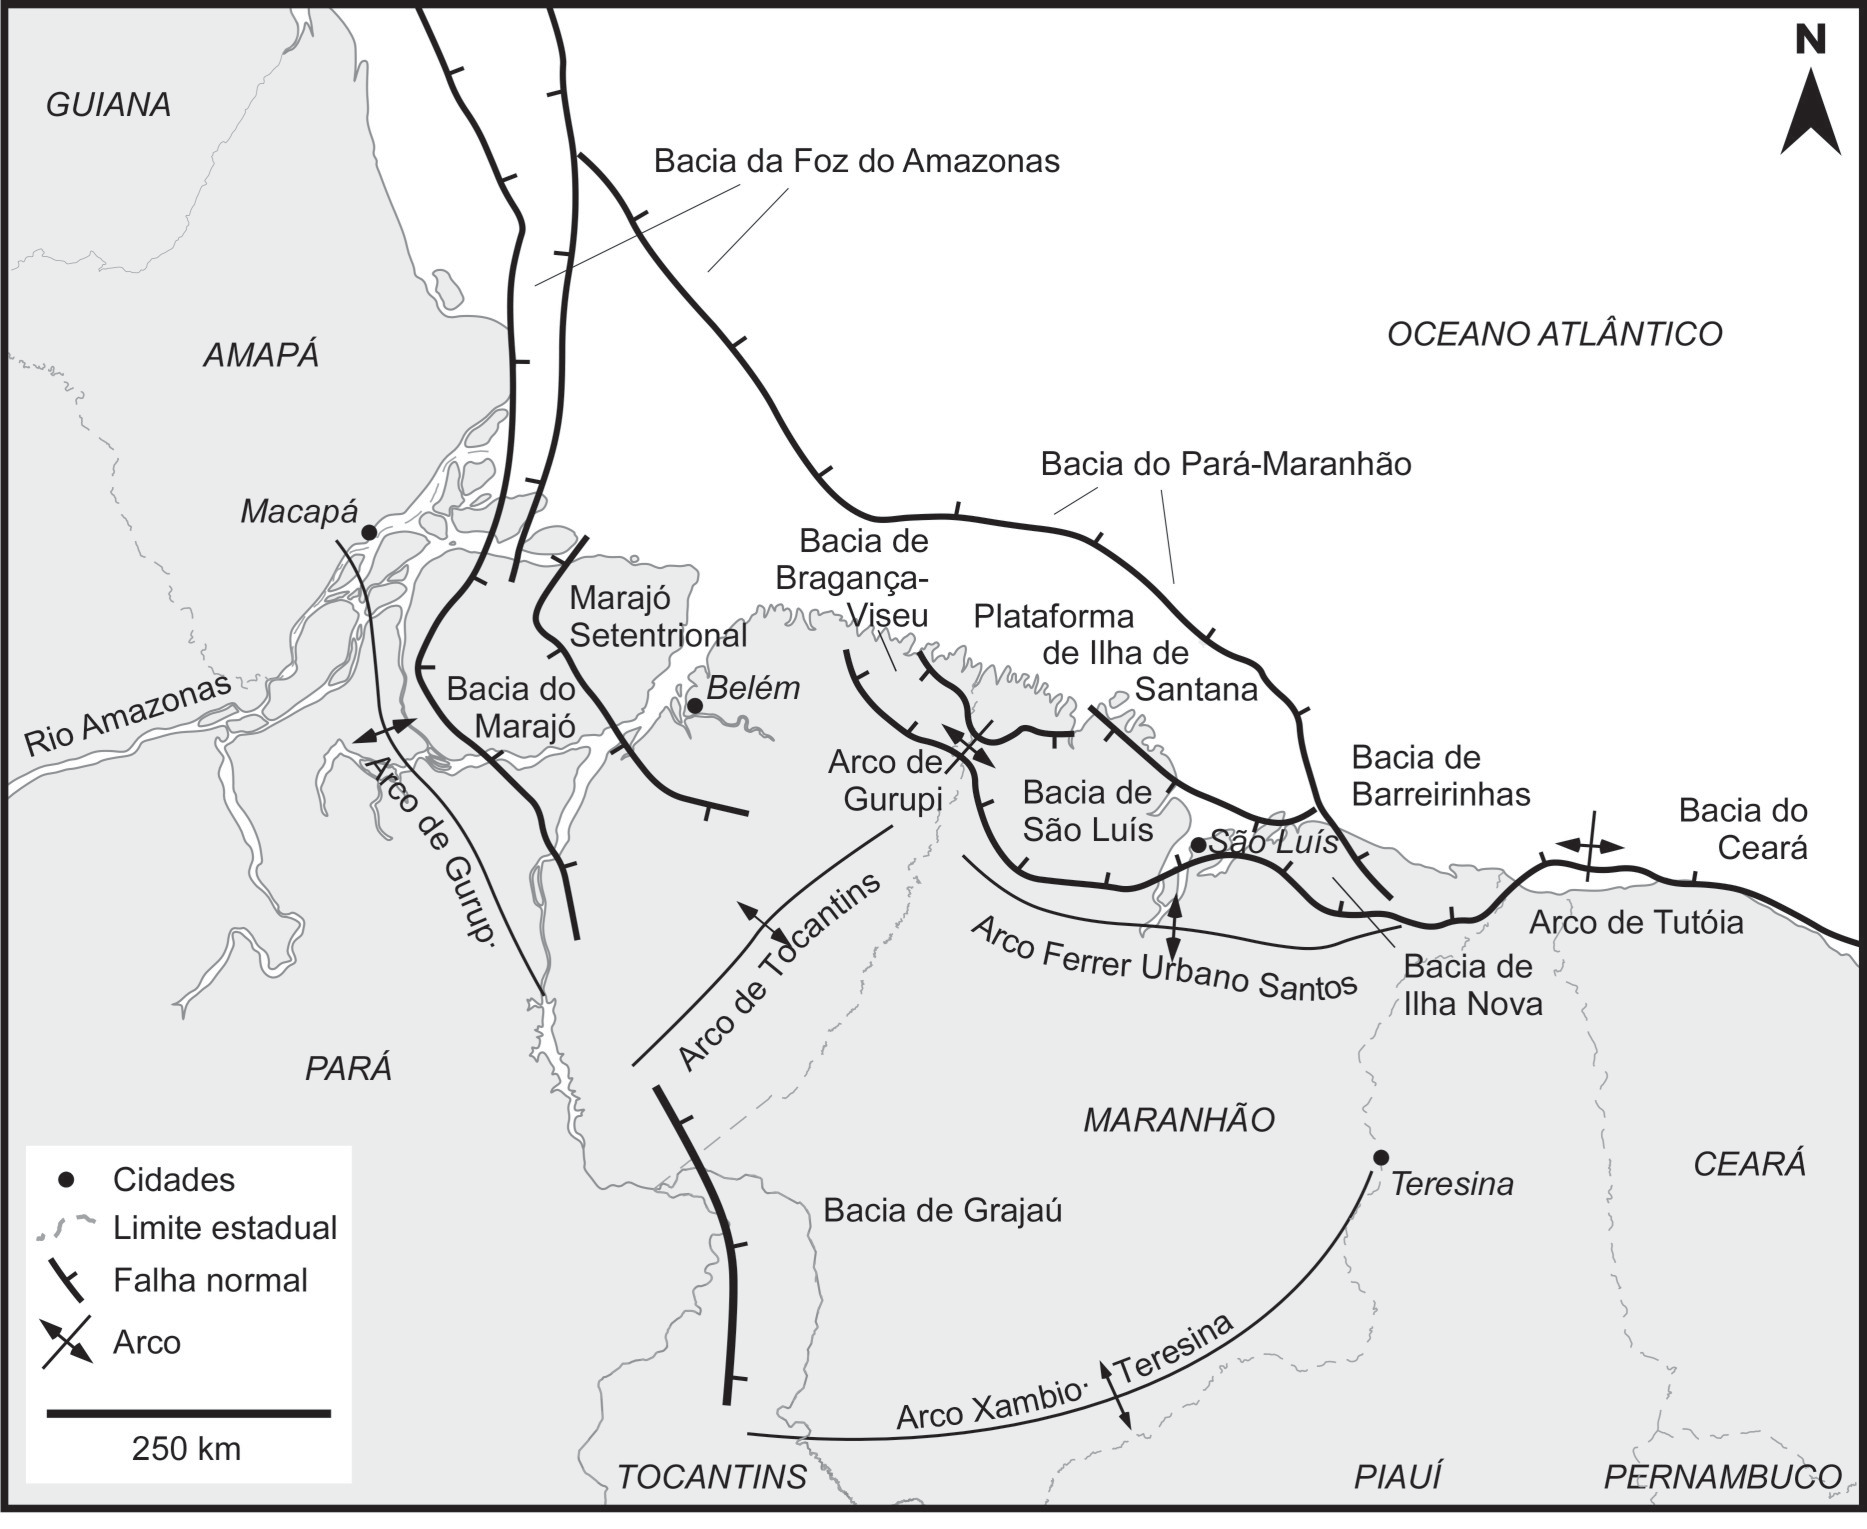
\includegraphics[width=0.36\textwidth]{figures/barreirinhas-geologic.png}
	}%
	\subfigure[]{%
	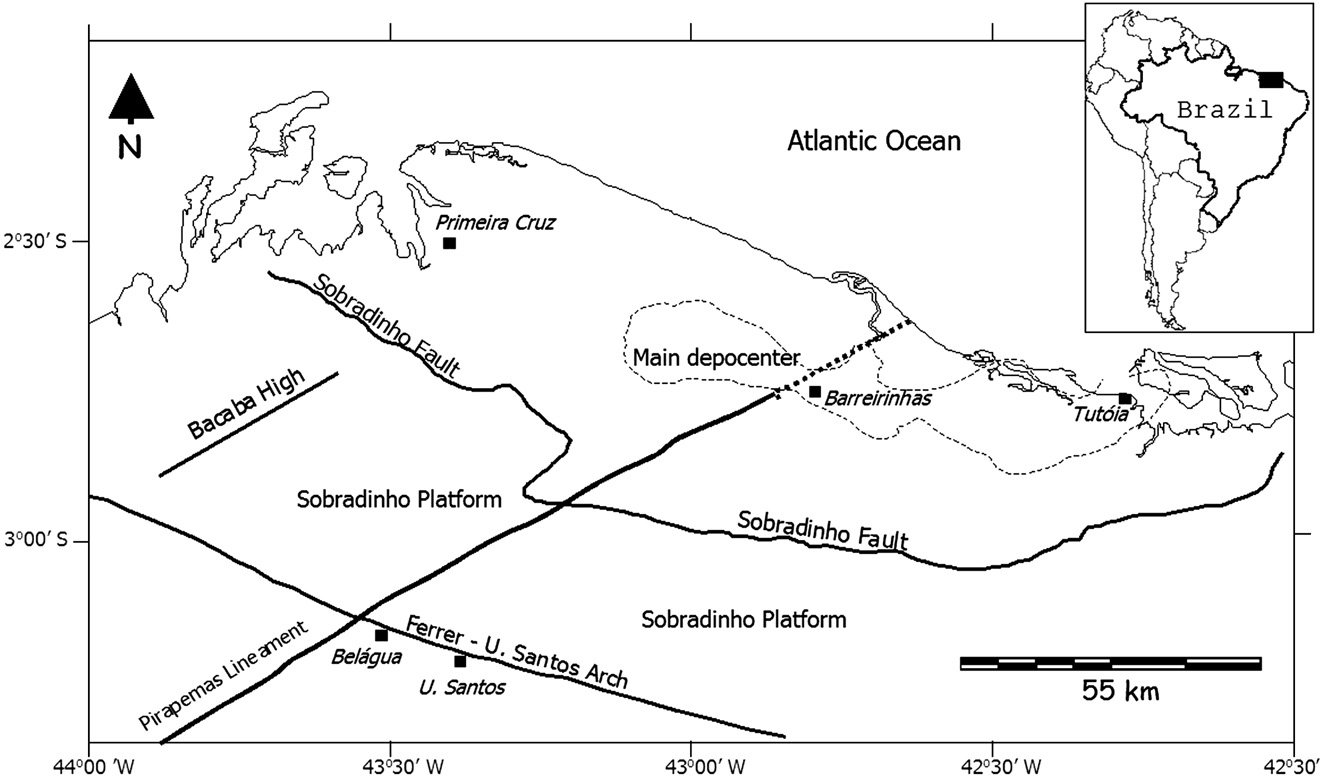
\includegraphics[width=0.55\textwidth]{figures/barreirinhas-depocenter.png}
	}
	\end{center}
	\caption{(a) Geologic map indicating arches, faults and lineaments. Source: \cite{soaresjunior2008evolucao}; (b) Simplified geologic map that shows main depocenter. Source: \cite{almeida2009quaternary}.}
	\label{fig1}
	\end{figure}
	
	Free-air anomaly map shows a two continuous lobes-sequence that represents a signature produced by crust geometric arrangement \cite{allen2013basin}. Gravity Bouguer anomaly has most negative areas representing São Luis and continental portion of Barreirinhas basins (see figure \ref{fig2}).
	
	\begin{figure}[ht!]
	\begin{center}
	\subfigure[]{%
	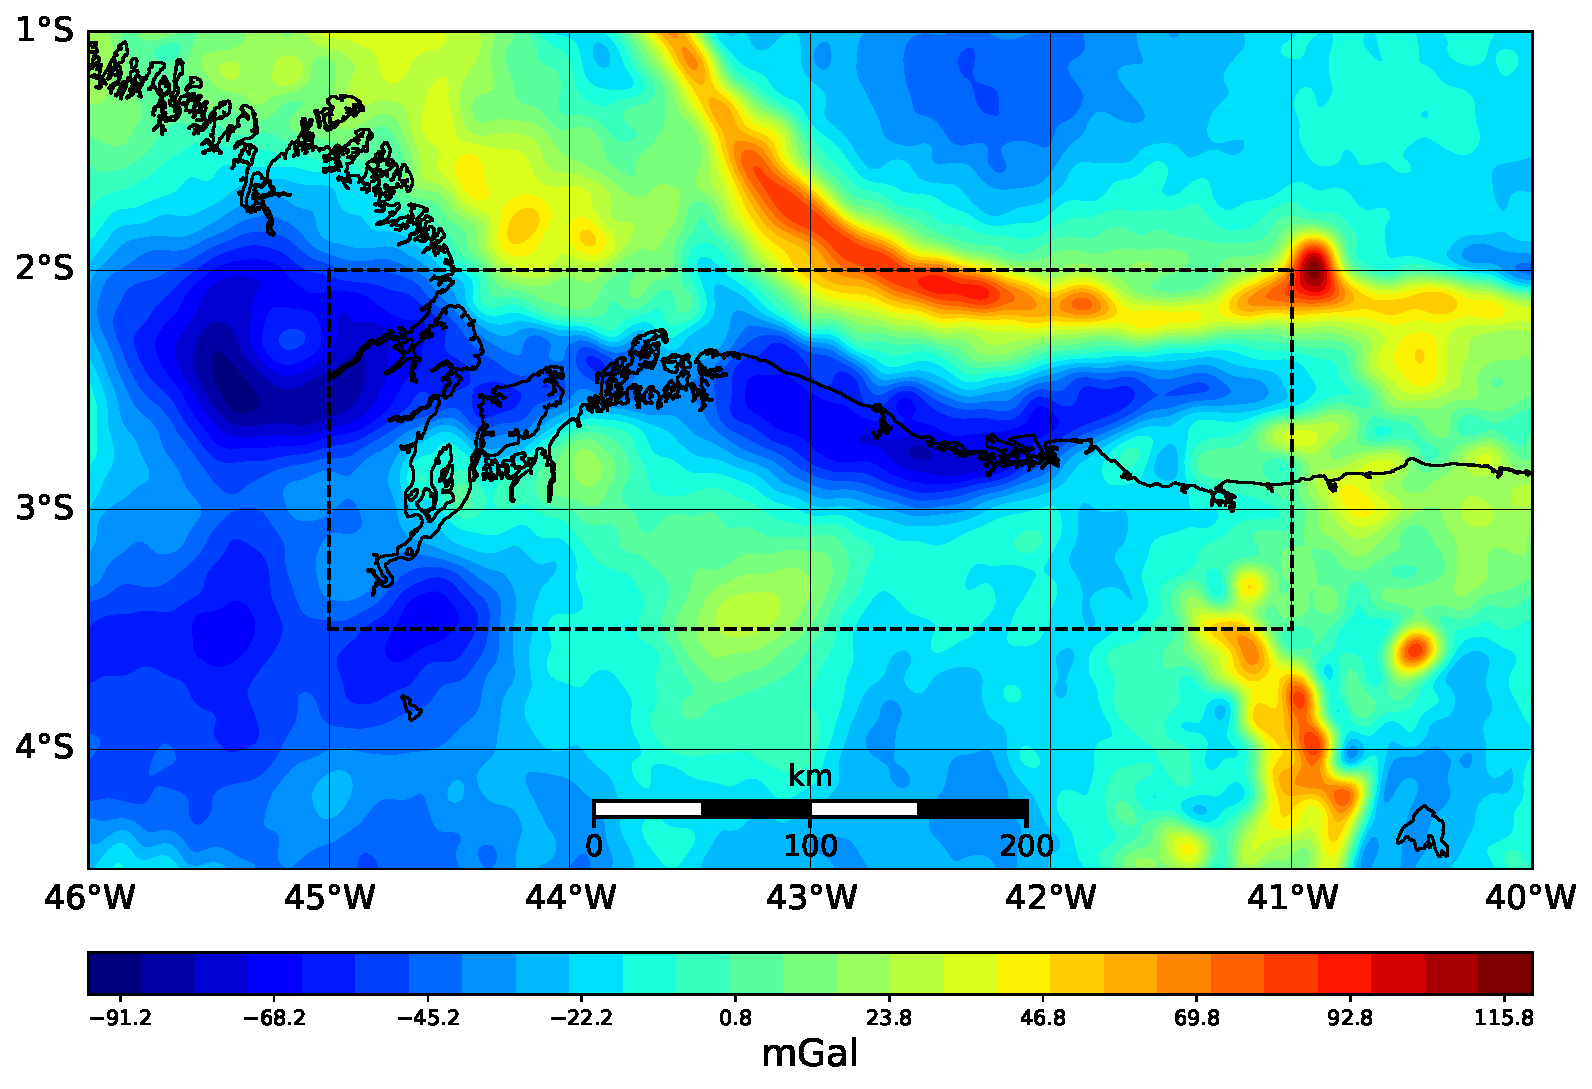
\includegraphics[width=0.975\textwidth]{figures/figure05-freeair.pdf}
	}\\
	\subfigure[]{%
	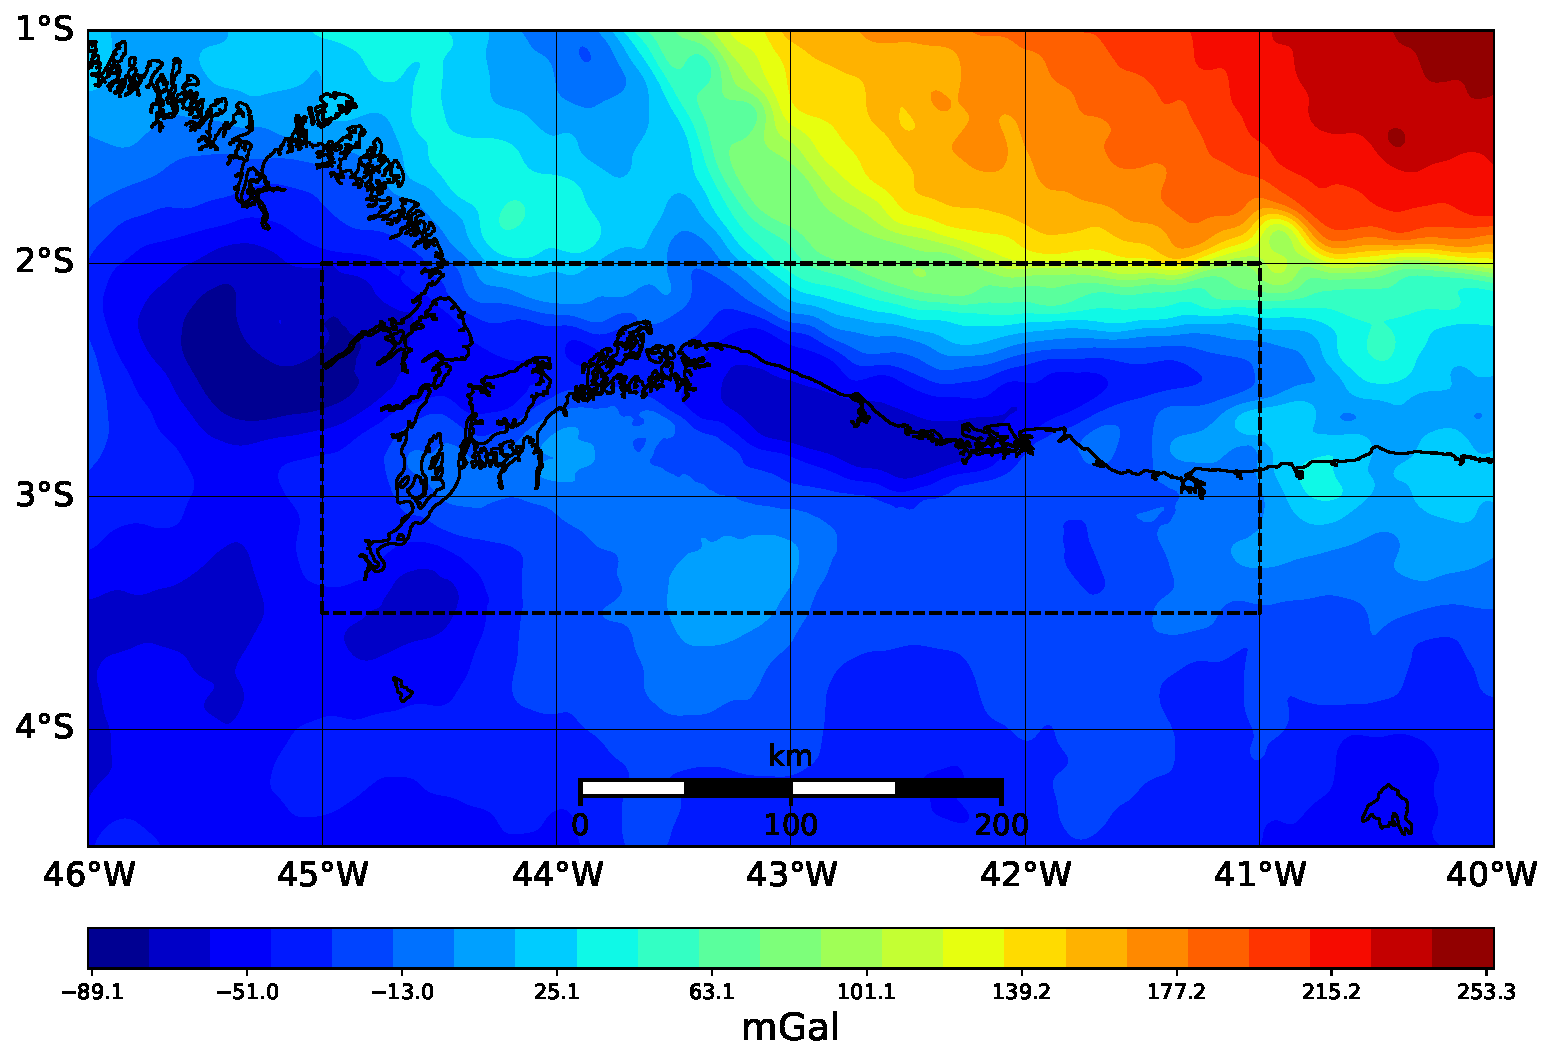
\includegraphics[width=0.975\textwidth]{figures/figure07-bouguer.pdf}
	}
	\end{center}
	\caption{(a) Free-air anomaly and (b) Simple Bouguer anomaly at Brazilian continental margin. Values provided by ICGEM. Black line represents the coastline.}
	\label{fig2}
	\end{figure}
	
	Crust top and bottom follow the continental margin behavior, once usually there is an abrupt transition zone between oceanic and continental crust (see figure \ref{fig3}).
	
	\begin{figure}[ht!]
	\begin{center}
	\subfigure[]{%
	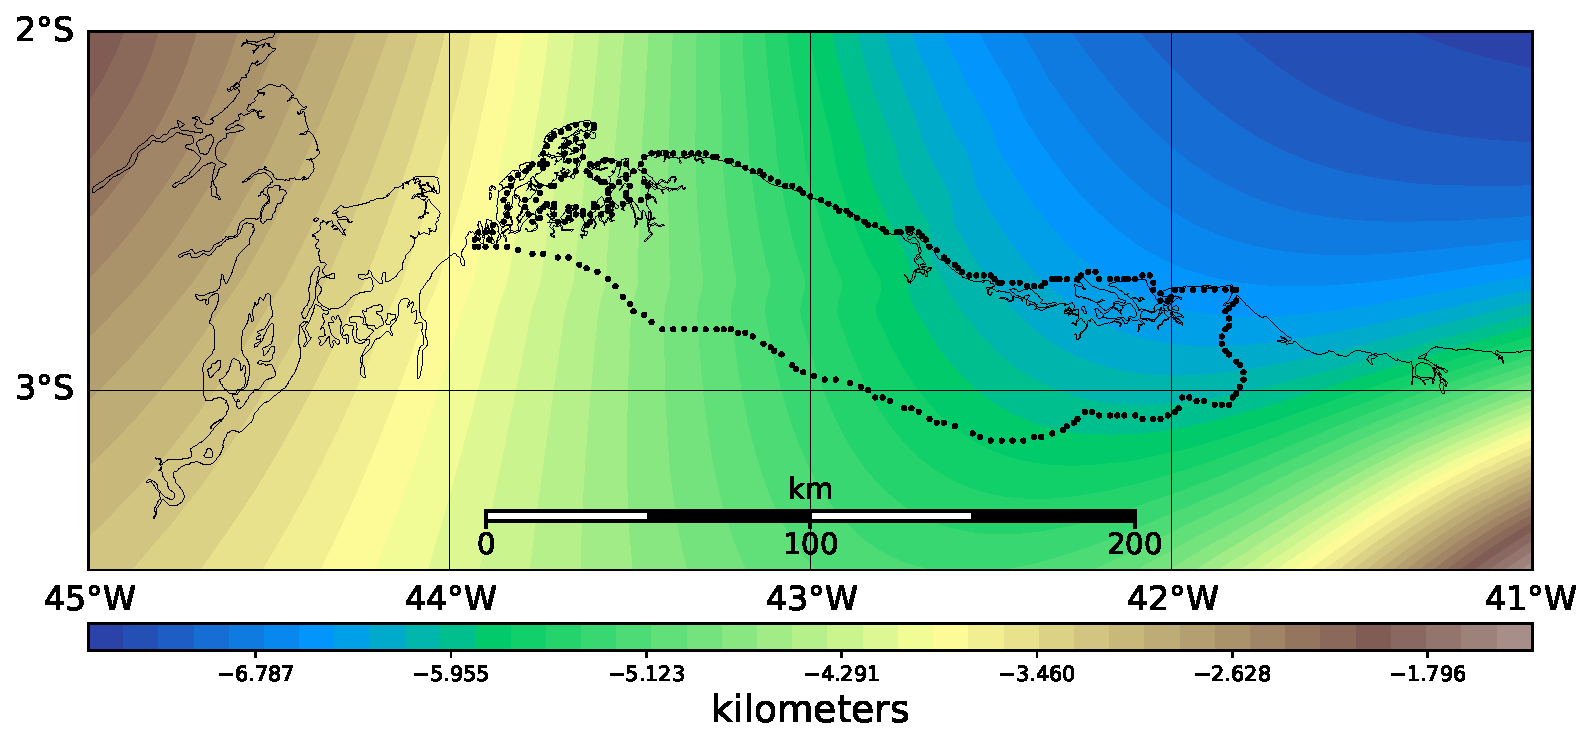
\includegraphics[width=0.456\textwidth]{figures/gemma-crust-top.pdf}
	}%
	\subfigure[]{%
	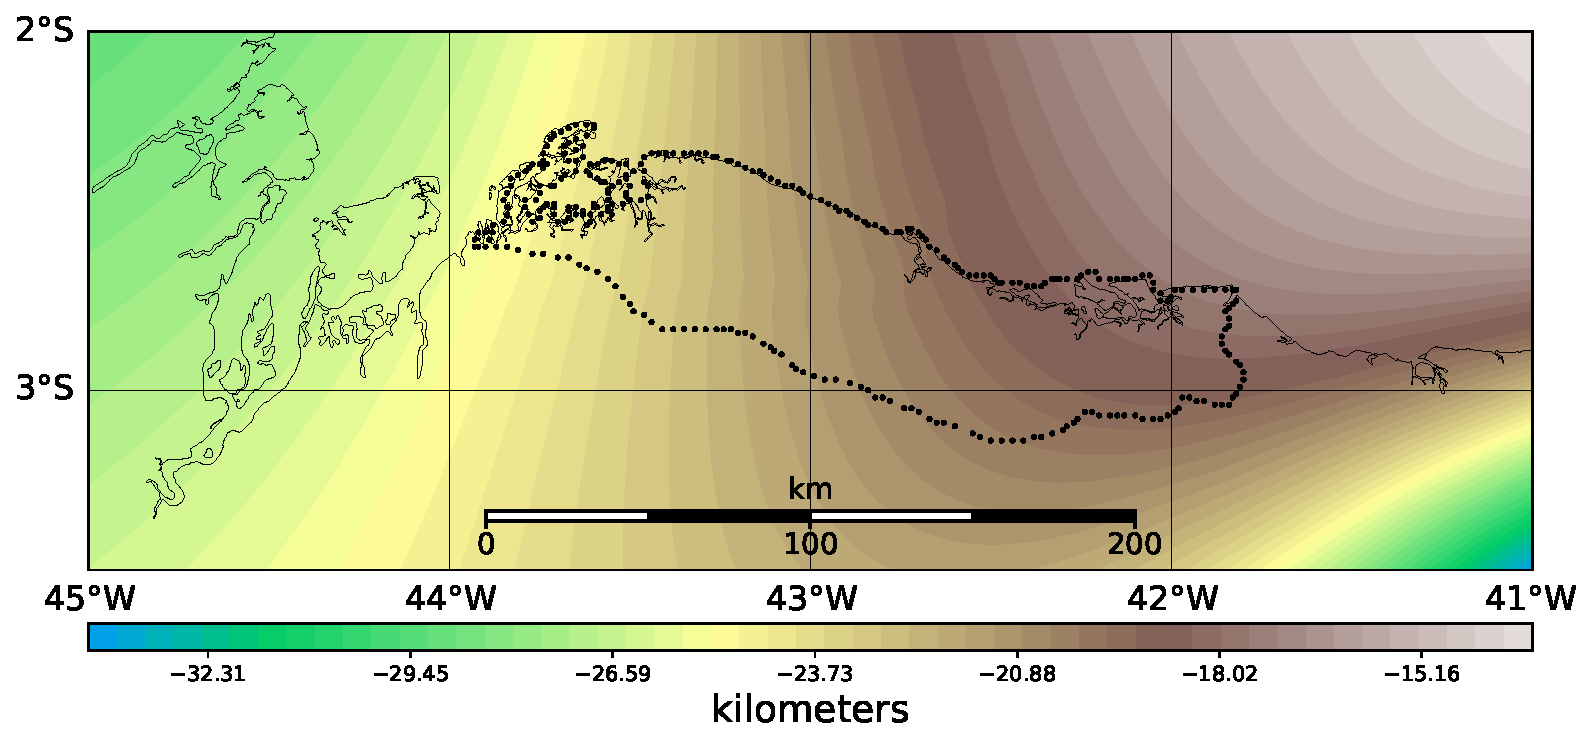
\includegraphics[width=0.456\textwidth]{figures/gemma-crust-bottom.pdf}
	}
	\end{center}
	\caption{Depht of (a) crust top and (b) crust bottom. Values provided by GEMMA model. Black line represents the coast line; dashed-line indicates Barreirinhas basin.}
	\label{fig3}
	\end{figure}
	
	\section*{\large Results}
	We present four solutions that were obtained. Regional anomaly maps show that all techniques were not able to estimate the true regional; on the contrary, crustal modeling was able to show the abrupt transition at continental margin (see figure \ref{fig4}).
	
	\begin{figure}[ht!]
	\begin{center}
	\subfigure[]{%
	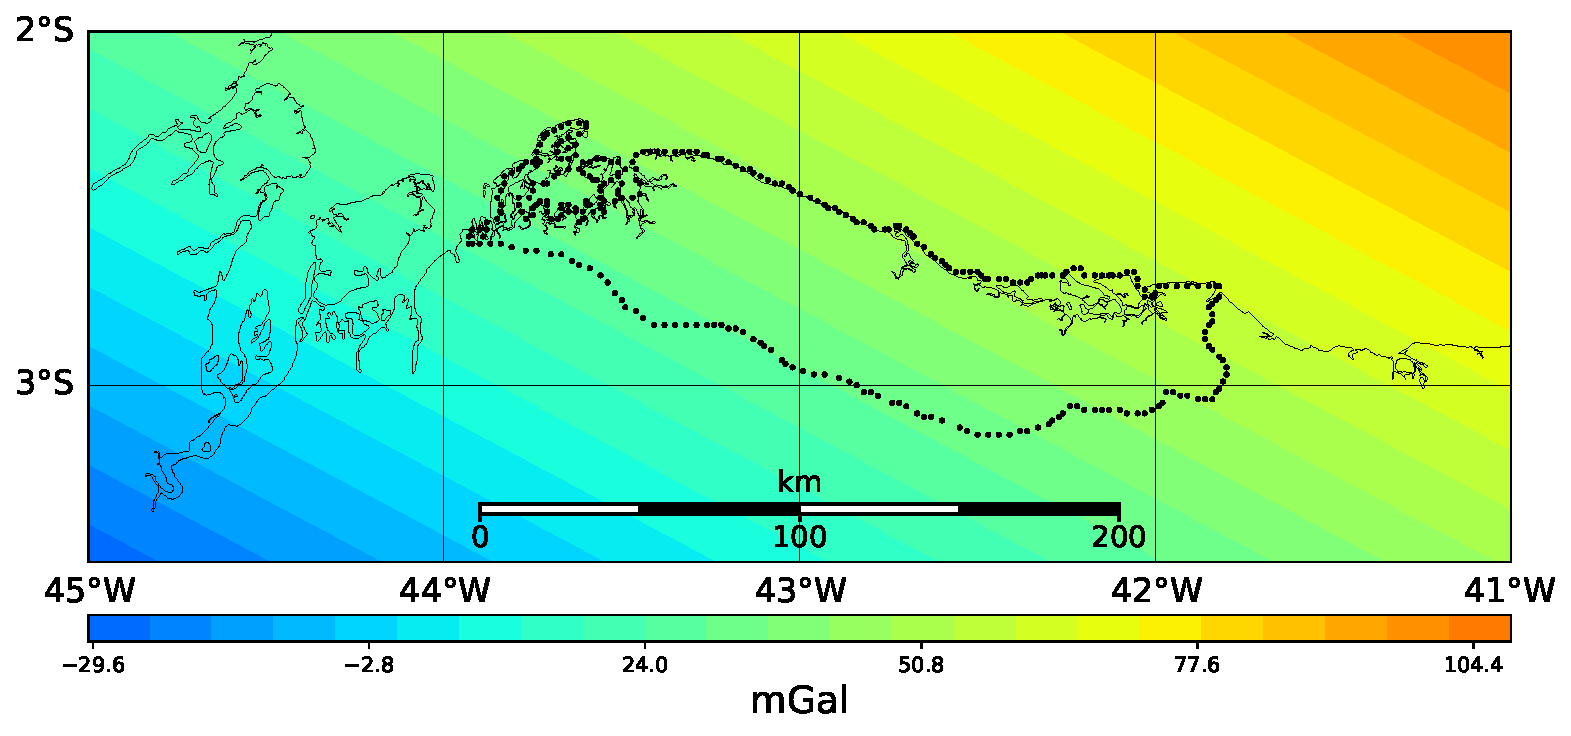
\includegraphics[width=0.456\textwidth]{figures/spectral01-regional.pdf}
	}%
	\subfigure[]{%
	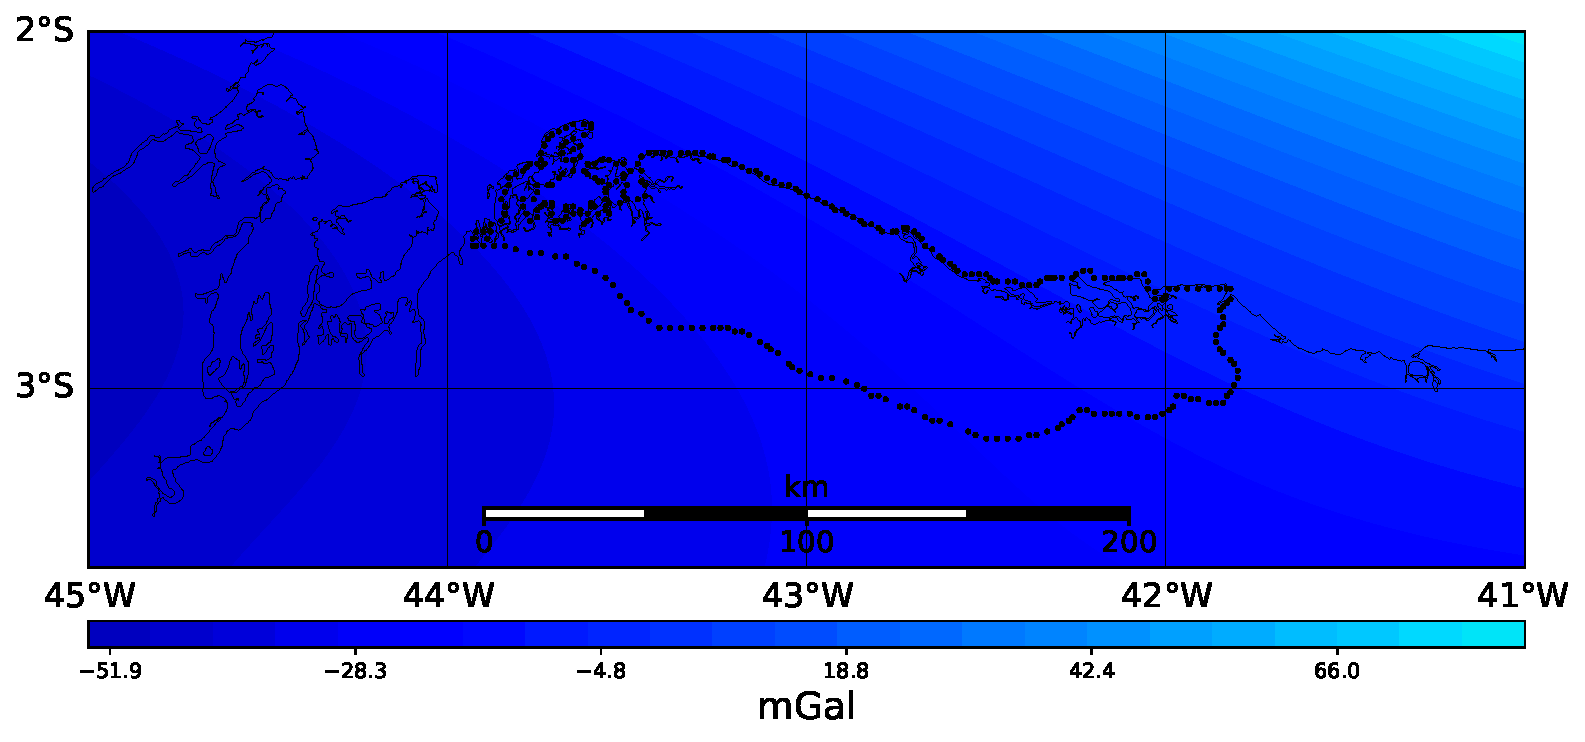
\includegraphics[width=0.456\textwidth]{figures/robust03-regional.pdf}
	}\\
	\subfigure[]{%
	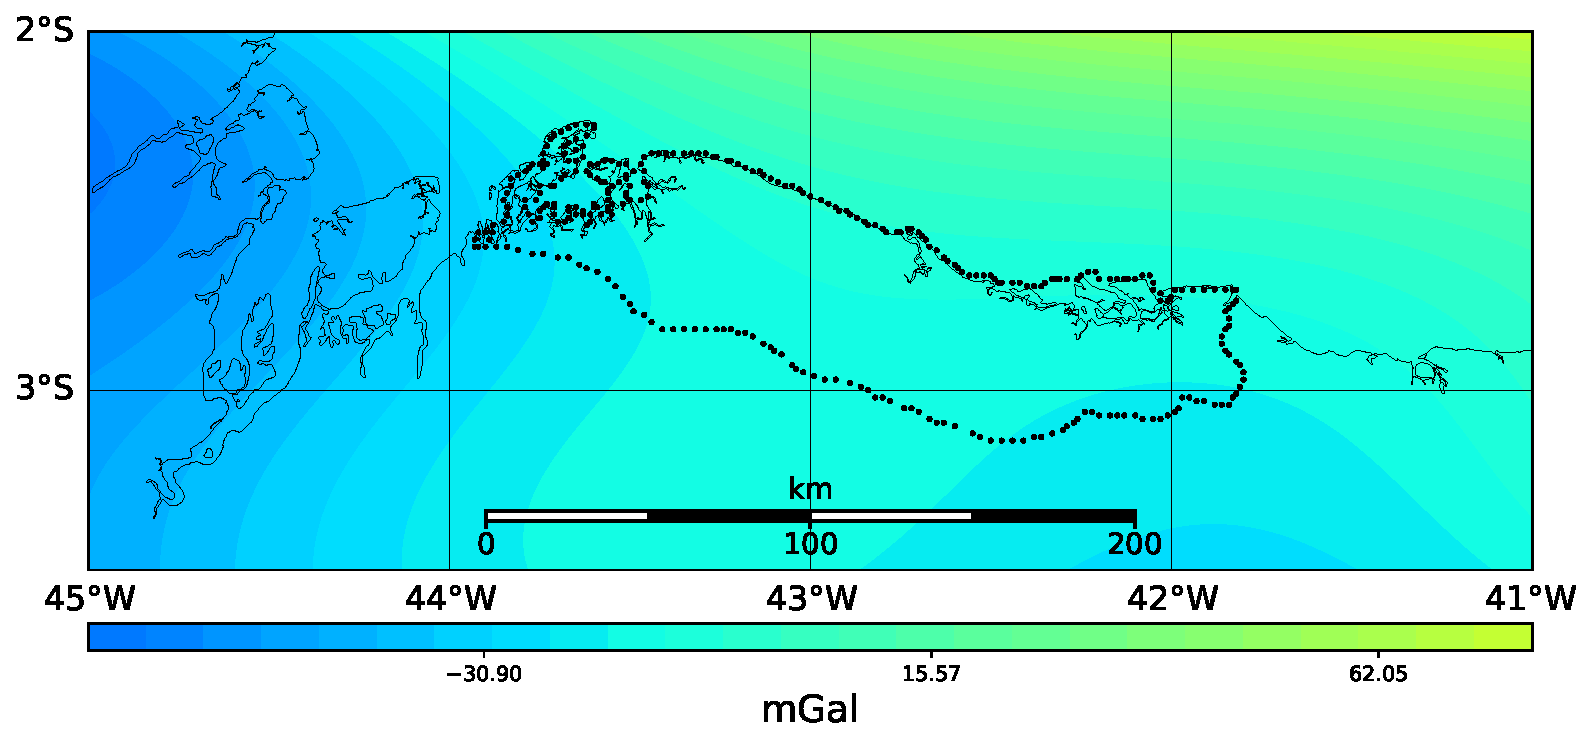
\includegraphics[width=0.456\textwidth]{figures/robust06-regional.pdf}
	}%
	\subfigure[]{%
	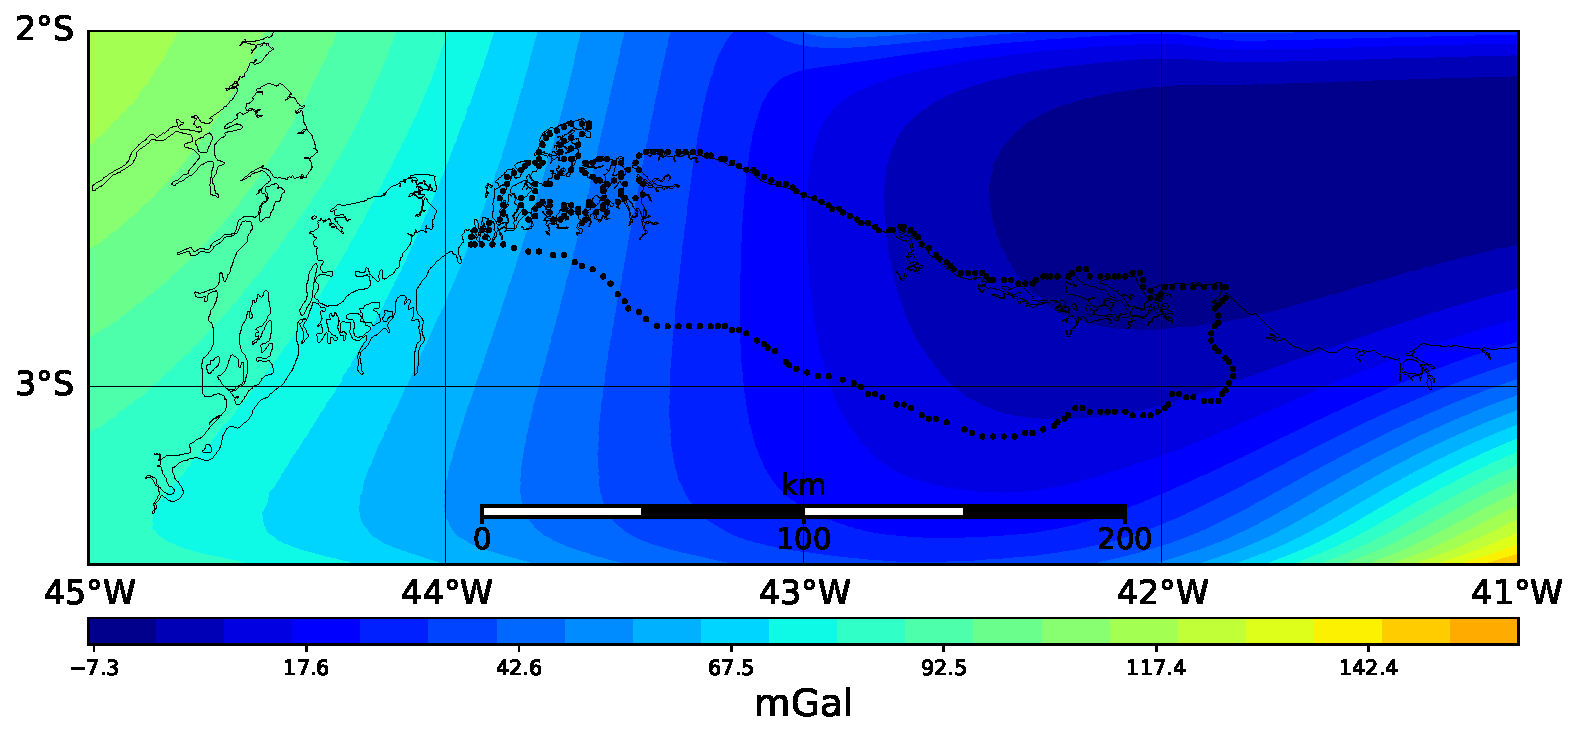
\includegraphics[width=0.456\textwidth]{figures/gemma01-regional.pdf}
	}
	\end{center}
	\caption{Regional signal obtained by: (a) spectral analysis; (b) third and (c) sixth polynomial degrees; (d) crustal modeling. Black line represents the coast line; dashed-line indicates Barreirinhas basin.}
	\label{fig4}
	\end{figure}
	
	Solutions of residual gravity anomaly from spectral analysis and robust polynomial shown similar amplitude and behavior. They were not able to adjust the basin contour. Residual signal from crustal modeling delimited the basin more effectively and shown possible unmapped faults (see figure \ref{fig5}). 
	All contour maps are blanked for positive values, once we assume residual signal usually is presented as negative.

	\begin{figure}[ht!]
	\begin{center}
	\subfigure[]{%
	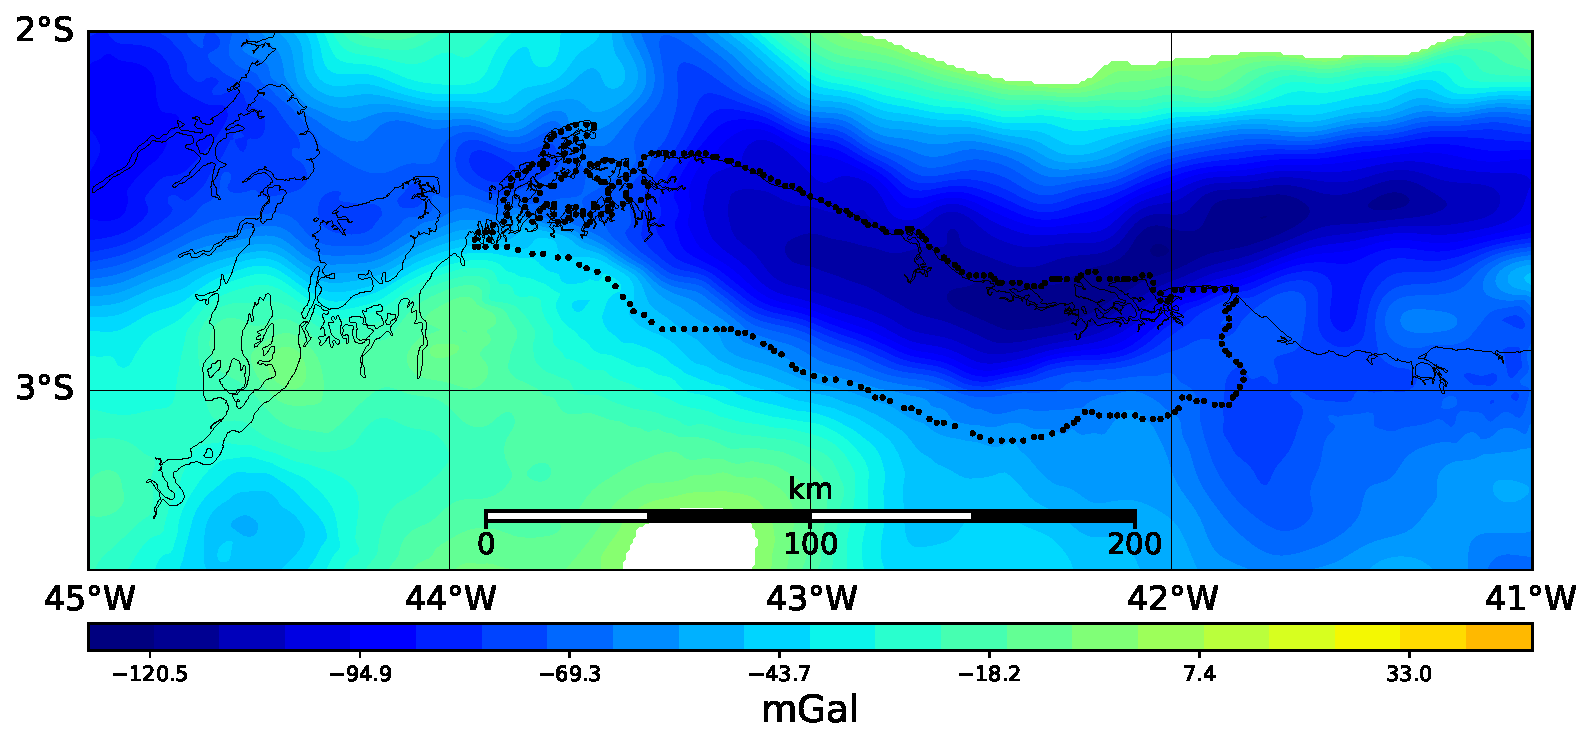
\includegraphics[width=0.456\textwidth]{figures/spectral01-residual(2).pdf}
	}%
	\subfigure[]{%
	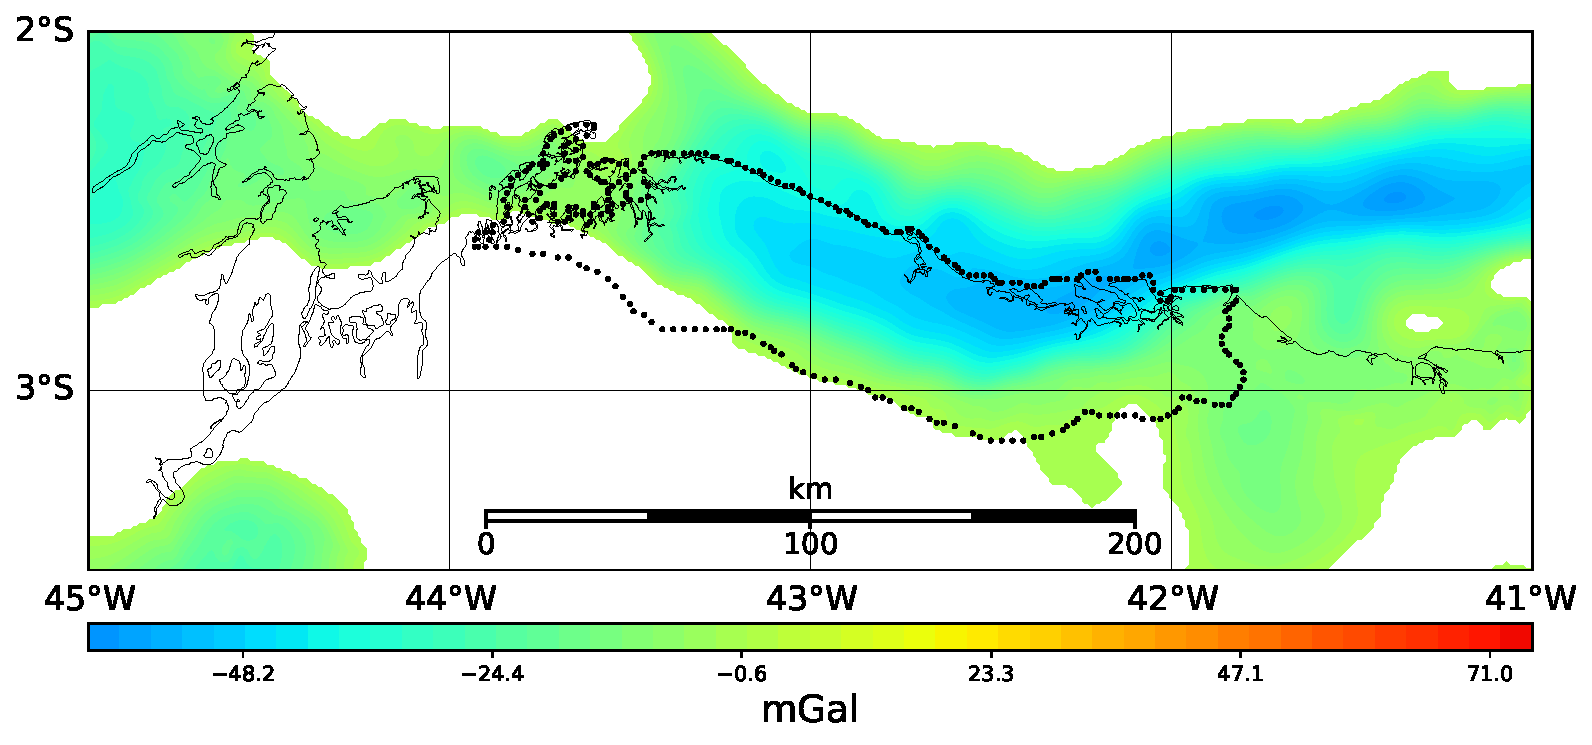
\includegraphics[width=0.456\textwidth]{figures/robust03-residual(2).pdf}
	}\\
	\subfigure[]{%
	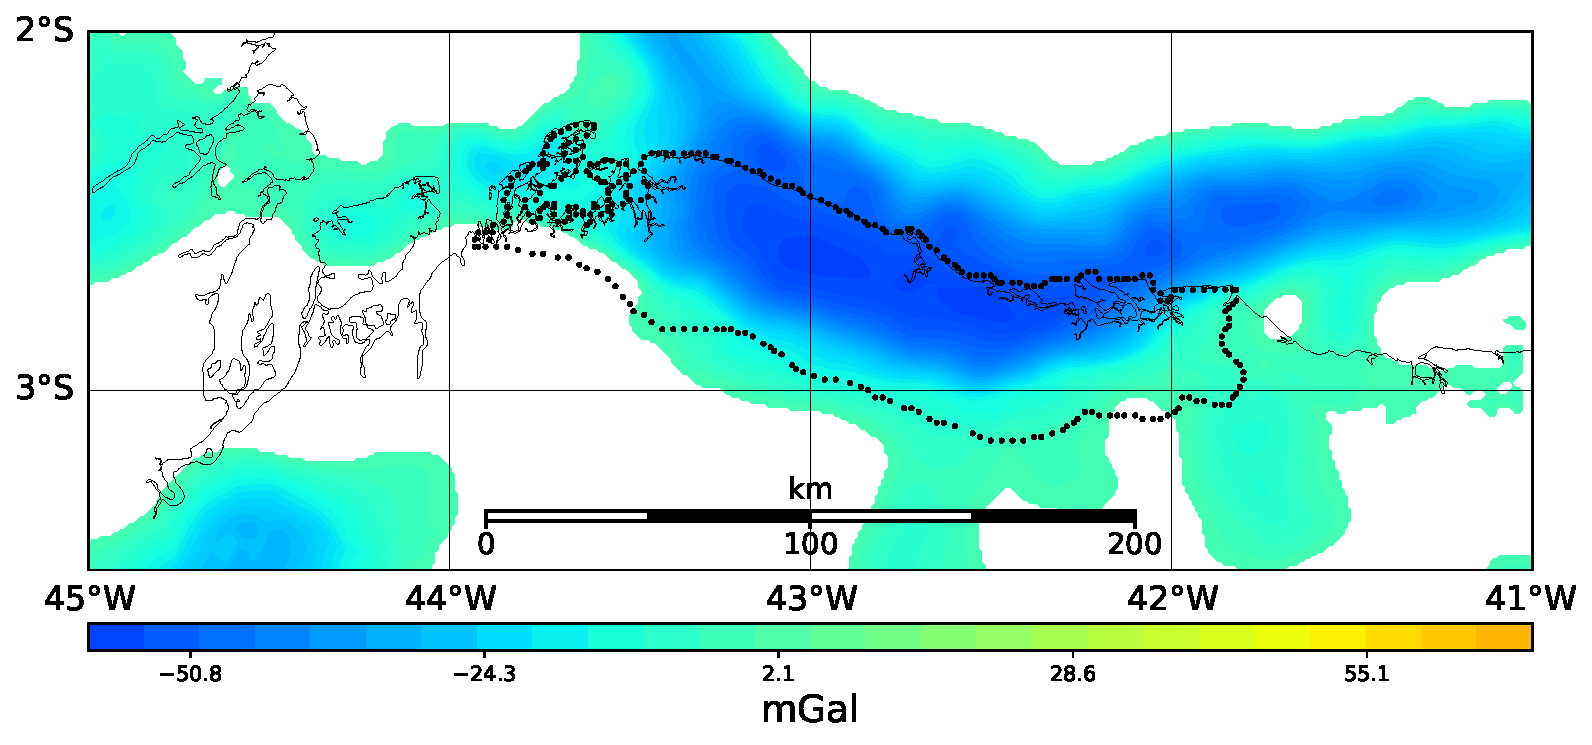
\includegraphics[width=0.456\textwidth]{figures/robust06-residual(2).pdf}
	}%
	\subfigure[]{%
	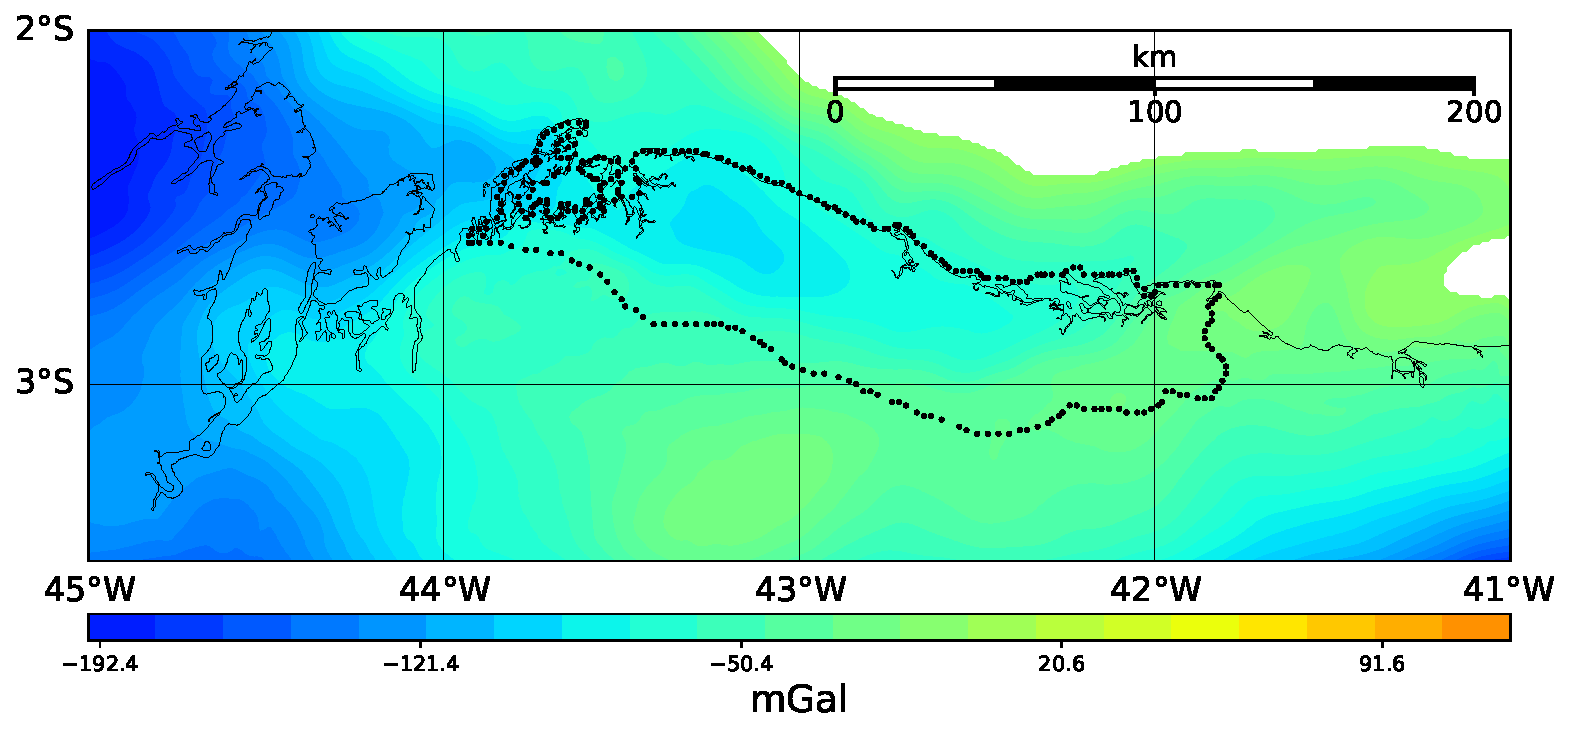
\includegraphics[width=0.456\textwidth]{figures/gemma01-residual(2).pdf}
	}
	\end{center}
	\caption{Residual signal through: (a) spectral analysis; (b) third and (c) sixth polynomial degrees; (d) crustal modeling. Black line represents the coast line; dashed-line indicates Barreirinhas basin.}
	\label{fig5}
	\end{figure}
	
	 It is possible affirm that residual anomaly is confined by the mapped faults and deepest basin region in the continental zone was identified, showing great correlation to the main depocenter cited in \cite{almeida2009quaternary}. Figure \ref{fig6} illustrates better the residual anomaly along with position of existing faults and lineaments.
	
	\begin{figure}
		\begin{center}
		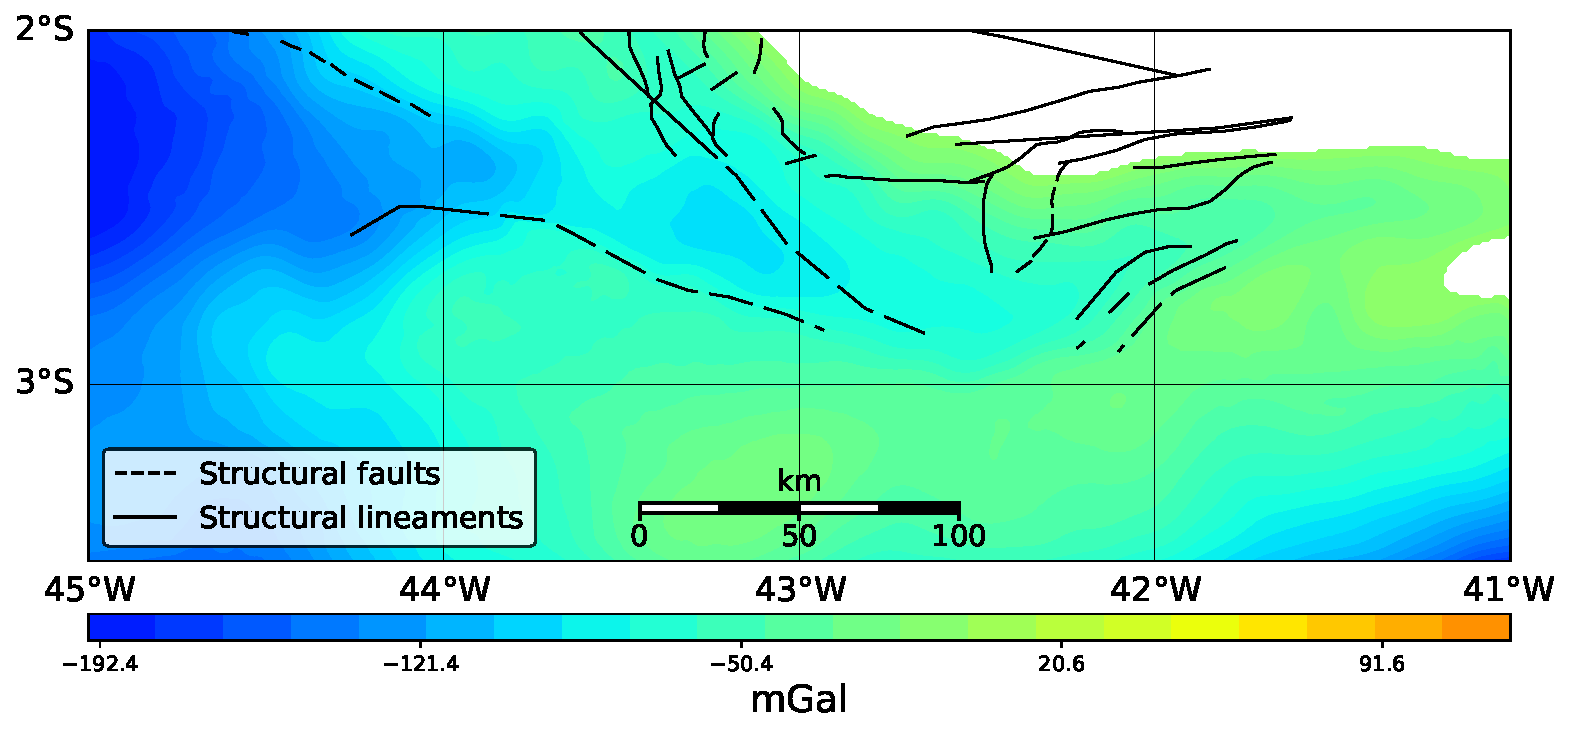
\includegraphics[width=0.885\textwidth]{figures/gemma01-residual(3).pdf}
		\end{center}
		\caption{Final residual gravity anomaly map of Barreirinhas basin. Black continuous and dashed lines indicate structural lineaments and faults, respectively.}
		\label{fig6}
	\end{figure}
		
	\section*{\large Discussion}
	\begin{itemize}
		\item[$i.$] Selecting best residual anomaly is a difficult task for interpreters;
		\item[$ii.$] Spectral analysis and robust polynomial fitting were not able to delineate the sedimentary basin;
		\item[$iii.$] Crust geometry causes a two-lobes shape in free-air anomaly usually hidden;
		\item[$iv.$] Once all crust attributes are present, crustal modeling has proved efficiency;
		\item[$v.$] Our approach mapped basin contour and depocenter;
		\item[$vi.$] For purpose of oil and gas prospecting, we strongly recommend this procedure for any sedimentary basins.
	\end{itemize}
	
	\section*{\large Acknowledgements}
	The authors would like to thank the Observatório Nacional (ON/MCTI) and CAPES for providing financial assistance.
	
	\bibliographystyle{plain}
	\bibliography{refs}
	\end{multicols}
\end{document}